\chapter{Research Methodology}
\label{ch:research-methodology}

\section{Research Model}
\label{sec:research-model}
The method of \textcite{Verschuren2016} is used for the research model.
	\begin{figure}[h]
		\centering
		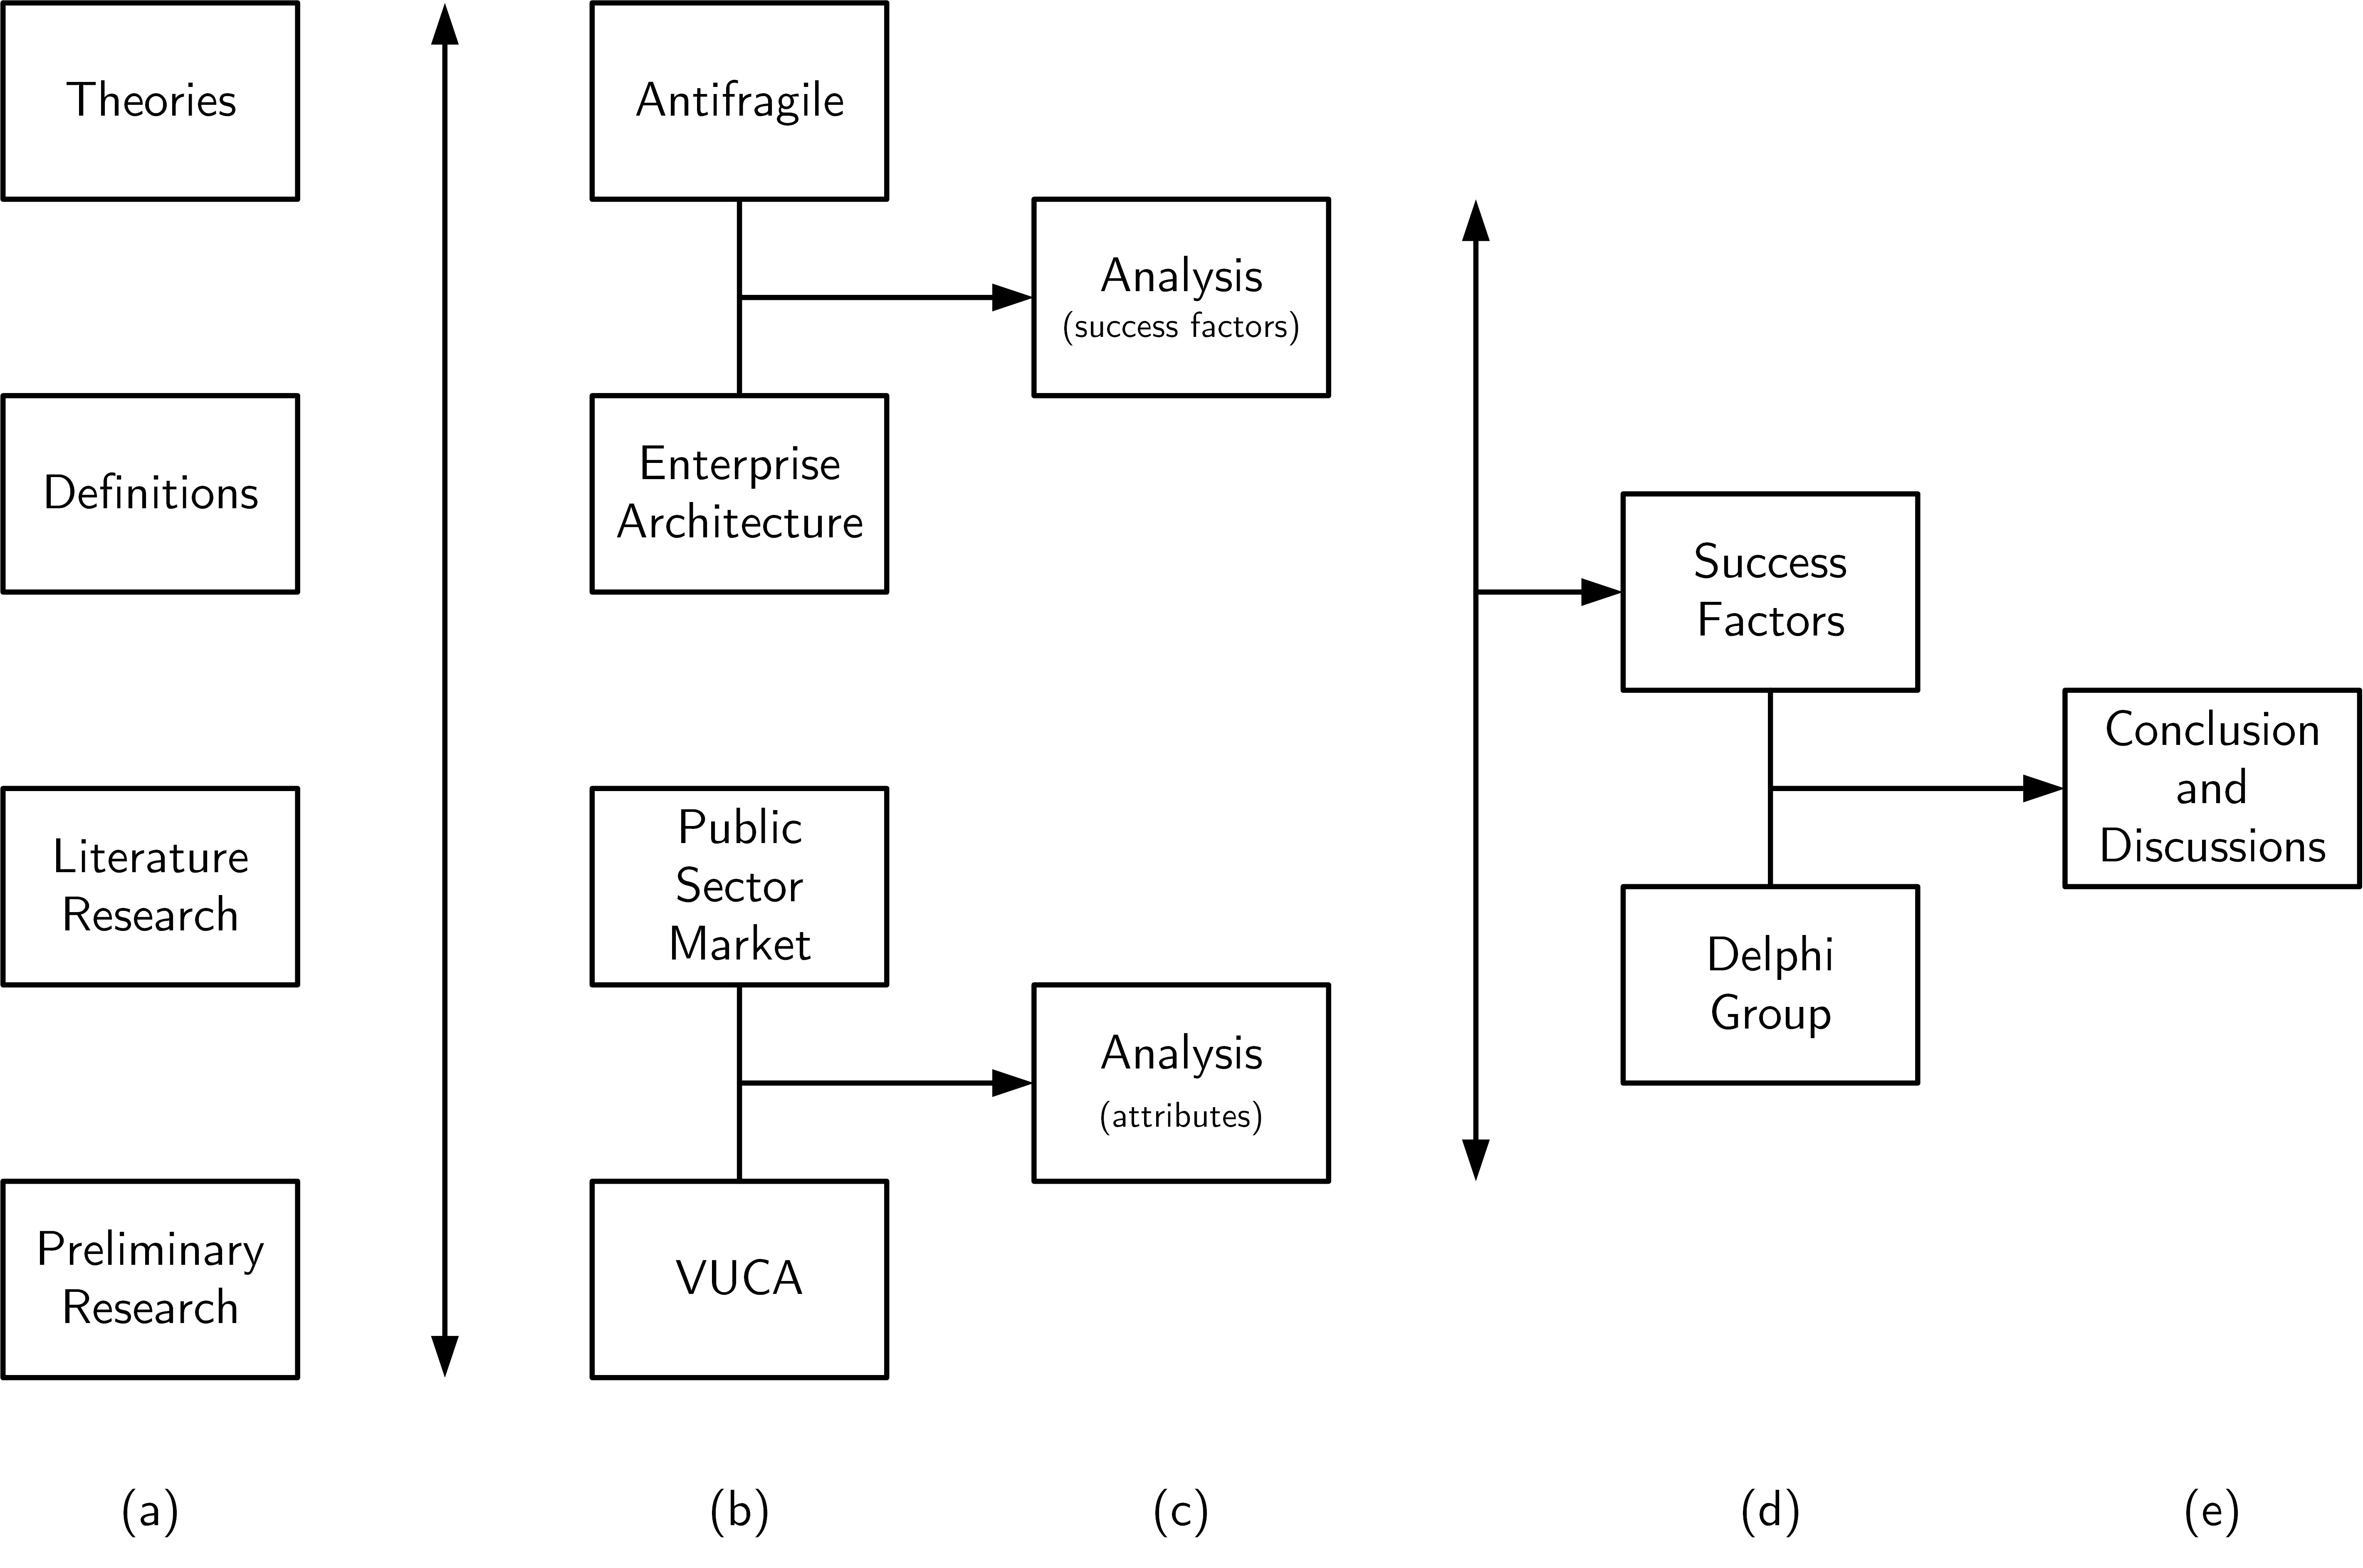
\includegraphics[width=12cm]{images/research-model.png}
		\caption[Research Model]{Research Model}
		\label{fig:research-model}
	\end{figure}

In the first phase of research (a), the researcher executes preliminary research and studies different theories and definitions of the involved concepts. The output of the first phase is the definitions and theories relevant to this research, such as \gls{antifragile}, \acrlong{ea}, the Public Sector market, and \acrshort{vuca}. In the second phase of research (b), the researcher confronts \gls{antifragile} with \acrlong{ea} and the Public Sector market with \acrshort{vuca}. The researcher uses interviews to validate the confrontation between the Public Sector Market with \acrshort{vuca}. The outcome of the second phase is the initiation of analysis on success factors of \acrlong{ea} relevant for contribution to \gls{antifragile} and analysis on attributes of the public sector market influenced by \acrshort{vuca} (c). In the fourth phase (d), the researcher uses the output of the analysis to confront the success factors with validation artefact through the Delphi Method to conclude and discuss his research (e).
\section{Research quality}
\label{sec:researchquality}
The researcher uses three frameworks to increase the rigorousness of the research as much as possible.
\begin{itemize}
	\item{Quality Principles of \textcite{Recker2013} (subsection \ref{sub:recker}).}
	\item{The FAIR Principles from Scientific Data (subsection \ref{sub:fair}).}
	\item{The Open Science Framework (subsection \ref{sub:osf}).}
\end{itemize}
\subsection{Quality Principles of Recker}
\label{sub:recker}
The first framework is that of \textcite[p. 16-17]{Recker2013} who uses four important principles:
\begin{itemize}
	\item{\textbf{Replicability} is a term that characterises the extent to which research procedures are repeatable. The principle states that the procedures by which research outputs are created should be conducted and documented in a manner that allows others outside the research team to independently repeat the procedures and obtain similar, if not identical, results.}
	\item{\textbf{Independence} is closely related to reliability. It concerns the extent to which the research conduct is impartial and freed from any subjective judgment or other bias stemming from the researcher or research team itself.}
	\item{\textbf{Precision} states that in all scientific research the concepts, constructs, and measurements should be as carefully and precisely defined as possible to allow others to use, apply, and challenge the definitions, concepts, and results in their own work.}
	\item{\textbf{Falsification} describes the logical possibility than an assertion, hypothesis, or theory can be contradicted by an observation or other outcome of a scientific study or experiment.}
\end{itemize}
\begin{remark}
	Howto falsify?
\end{remark}
\subsection{Fair Principles}
\label{sub:fair}
In 2016, the 'FAIR Guiding Principles for scientific data management and stewardship' were published in Scientific Data. The authors intended to provide guidelines to improve the Findability, Accessibility, Interoperability, and Reuse of digital assets. The research is using the FAIR Principles\footnote{\url{https://www.go-fair.org/fair-principles/}} to increase the quality of the published thesis.
\begin{itemize}
	\item{\textbf{Findable.} The first step in (re)using data is to find them. Metadata and data should be easy to find for both humans and computers. Machine-readable metadata are essential for automatic discovery of datasets and services. The thesis, research and used datasets are containing keywords, links, and structures that can be indexed.}
	\item{\textbf{Accesible.} Once the user finds the required data, she/he/they need to know how can they be accessed. The thesis, research and used datasets are published on GitHub, Zenodo, and Researchgate based on Open Access. The researcher created objects containing a location on where the data can be acquired if it cannot be published because of author rights.}
	\item{\textbf{Interoperable.} The data usually need to be integrated with other data. In addition, the data need to interoperate with applications or workflows for analysis, storage, and processing. This principle is not relevant for this research. The data are qualitative data sets based on literature, interviews, and questionnaires.}
	\item{\textbf{Reusable.} The ultimate goal of FAIR is to optimise the reuse of data. To achieve this, metadata and data should be well-described so that they can be replicated and/or combined in different settings. The thesis, research and used datasets are published under the \href{https://creativecommons.org/licenses/by-sa/4.0/}{\ccbysa\ CC-BY-SA 4.0 license.} It is allowed that the thesis, research, and datasets are shared and are adapted (even commercially) as long as the original author is attributed and the possible derivate is published under the same license.}
\end{itemize}
\subsection{The Open Science Framework}
\label{sub:osf}
One of the starting points of the research is Open Science. The idea behind Open Science is to allow scientific information, data and outputs to be more widely accessible (Open Access) and more reliably harnessed (Open Data) with the active engagement of all the stakeholders (Open to Society) \parencite{UNESCO2020}. The Center for Open Science\footnote{{\url{https://www.cos.io/}}} supports this way of research by supplying guidelines and even a toolkit. For this research the toolkit is used to support Open Access, Open Data and Open to Society. One of the tools in the toolkit is a reference model to select tools for the four main phases of research: Search and Discover, Design Study, Collect and Analyse Data, and Publish Reports. The researcher uses this reference model in section \ref{sec:researchinfraandtooling}. Using this framework will help in achieving replicability, precision, and reusability.
\section{Research approach}
\label{sec:researchapproach}



What is literature saying about the Public Sector Market?
What is literature saying about \acrlong{ea}?
What is literature saying about the success factors of Enterprise Architecture?
What does literature say about antifragile?
How can the success factors of \acrlong{ea} contribute to becoming antifragile?


What are the success factors of \acrlong{ea} for \gls{antifragility} in the public sector market?

\section{Delphi Method}
For the Delphi Group participants see appendix~\ref{app:delphigroupparticipants} \\%

What about the sample size? Normally Delphi is about 100+. What about this research. How large should the sample size be for a qualitative result?\
Answer of sample size 12 to 18 (stated by promotor)\\
The result of the research of \textcite[p. 404]{Diamond2014} states a median of 75\% to determin consensus.
\begin{remark}
	After email conversation with Hans. I decided on 12 tot 18 participants.
\end{remark}


\section{Literature research}
For the literature research two methods are used. The first method is (foward and backward) snowballing already found literature. The second method is the use of scientific (online) libraries. The used libraries are:
\begin{itemize}
	\item{Web of Science}
	\item{Research Gate}
	\item{Google Scholar}
\end{itemize}

\noindent A predefined collection of search strings is used for the search with scientific libraries.

\subsection{Search strings}
The following search strings are used for finding literature with the scientific libraries. Not only the full concept name is used but also the abbreviations (eg. Independent Software Vendor and ISV, Enterprise Architecture and EA).\\

	\noindent
	\begin{tabular}{p{0.5\textwidth}p{0.5\textwidth}}
		\textbf{\acrlong{ea}} & \\
		Enterprise Architecture Antifragile	&	Search String 2\\%
		Search String 3	&	Search String 4\\%
	\end{tabular}

\vspace{\baselineskip}

	\noindent
	\begin{tabular}{p{0.5\textwidth}p{0.5\textwidth}}
		\textbf{\Gls{antifragile}} & \\
		antifragile robust agile resilient	&	Search String 2\\%
		Search String 3	&	Search String 4\\%
	\end{tabular}

\vspace{\baselineskip}

	\noindent
	\begin{tabular}{p{0.5\textwidth}p{0.5\textwidth}}
		\textbf{\acrlong{isv}} & \\
		Independent Software Vendor antifragile	& Independent Software vendor resilient\\%
		Independent Software Vendor Public Sector	&	Independent Software Vendor Enterprise Architecture\\%
	\end{tabular}

\vspace{\baselineskip}

	\noindent
	\begin{tabular}{p{0.5\textwidth}p{0.5\textwidth}}
		\textbf{Public Sector} & \\
		Difference public and private sector &	Public Sector antifragile\\%
		Public Sector resilient	&	Search String 4\\%
	\end{tabular}

\vspace{\baselineskip}

	\noindent
	\begin{tabular}{p{0.5\textwidth}p{0.5\textwidth}}
		\textbf{Enterprise Architeture \& Antifragile} & \\
		Search String 1	&	Search String 2\\%
		Search String 3	&	Search String 4\\%
	\end{tabular}

\paragraph{Enterprise Architect \& Antifragility}


\paragraph{Public Sector Market \& Independent Software Vendor}

\subsection{Criteria for admission of literature}
It is essential that the literature must help to develop the knowledge necessary to conduct the research. But before the literature can be used the quality of the literature must be evaluated. For evaluating the literature on the usability for this research the criteria accuracy, authority, objectivity, currency, and coverage is used\footnote{\url{https://libguides.library.cityu.edu.hk/litreview/evaluating-sources/}}.



\section{Research infrastructure and tooling}
\label{sec:researchinfraandtooling}
For selecting the suitable instruments for the research, the Open Science Framework\footnote{\url{https://www.cos.io/products/osf}} is used. The Open Science Framework consists out of 4 stages in a research project. Those stages are: ''Search and Discover, Design Study, Collect and Analyse, and Publish Reports.'' The Open Science Framework proposes specific infrastructure and tools per stage. The transparency in the used infrastructure and tools increases the quality of the research. It increases the replication factor, findability, accessibility, interoperability, and reusability.
\begin{figure}[H]
	\centering
	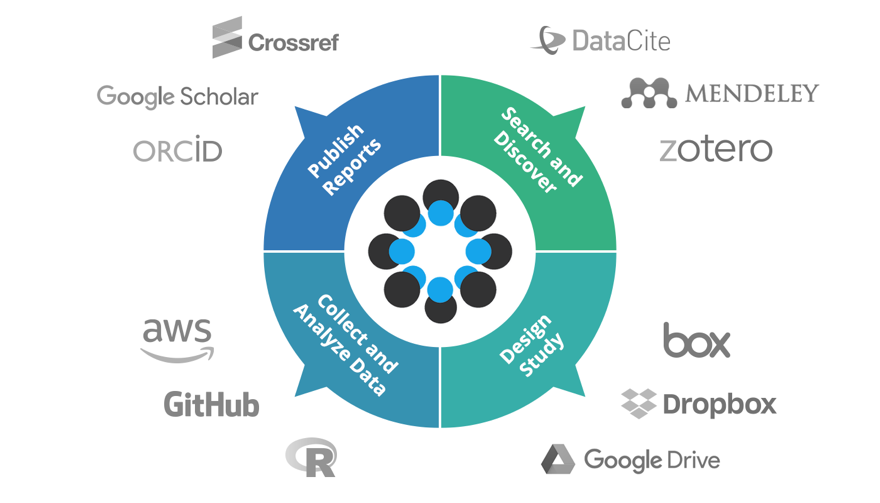
\includegraphics[width=0.7\linewidth]{images/osfframework}
	\caption[Open Science Framework]{Open Science Framework}
	\label{fig:osfframework}
\end{figure}
\subsection{Thesis creation}
The student used his corporate laptop (Dell Latitude 7200 2-in-1\footnote{\url{https://www.dell.com/en-us/work/shop/dell-laptops-and-notebooks/latitude-7200-2-in-1-laptop/spd/latitude-12-7200-2-in-1-laptop}}) with Windows 10 Professional installed for creating the thesis. The thesis is created with the markup language \LaTeX\footnote{\url{https://www.latex-project.org/}}. The used typesetting environment is TexLive\footnote{\url{https://www.tug.org/texlive/}} with the document type of ''Report'' from KOMA-Script\footnote{\url{https://ctan.org/pkg/koma-script}}. TexStudio\footnote{\url{https://www.texstudio.org/}} is the used \LaTeX\ Editor. It supports syntax-highlighting, has an integrated viewer, reference checking and numerous wizards. For the creation and administration of references Bib\LaTeX\footnote{\url{https://ctan.org/pkg/biblatex/}} is used with the reference manager JabRef\footnote{\url{https://www.jabref.org/}} with the citation style of APA 7th Edition\footnote{\url{https://apastyle.apa.org/}} and with web browser integration. The files are stored on a personal Dropbox\footnote{\url{https://www.dropbox.com/}} that is used by GitHub Desktop\footnote{\url{https://desktop.github.com/}} to synchronise with a public GitHub repository\footnote{\url{https://github.com/JRBliekendaal/master-thesis}}. GitHub\footnote{\url{https://github.com/}} is used for source control but also for reviewing and discussing the topics with the (Co-)Promotor and the planning of the master thesis project. The thesis source files are copied to an Amazon S3 Blob\footnote{\url{https://aws.amazon.com/s3/}} for backup. The backup rotation is seven versions. Cloudberry Explorer Freeware for Amazon S3\footnote{\url{https://www.msp360.com/explorer/windows/amazon-s3.aspx}} is used for backup. Grammarly\footnote{\url{https://www.grammarly.com}}, with the paid subscription service, checks the thesis for spelling, grammar,  style, and plagiarism. The used goals for Grammarly are audience=knowledgeable, formality=formal, and domain=academic. Microsoft Visio Professional\footnote{\url{https://www.microsoft.com/en-ww/microsoft-365/visio/}} is used to create figures. The GitHub repository contains all the sources.
\subsection{Research administration}
\label{tbresearchadministration}
The research administration, which includes documentation containing privacy-sensitive information, like the name and contact information of the Delphi Group participants, is stored on a non-public GitHub Repository\footnote{\url{https://github.com/JRBliekendaal/master-thesis-administration}}. The private GitHub Repository is also for staging thesis parts that still need to be anonymised. For taking notes Leuchtturm1917\footnote{\url{https://www.leuchtturm1917.us/notebook-classic.html}} Notebooks are used with mechanical pencils of Faber-Castell\footnote{\url{https://www.fabercastell.com/products/tk-fine-vario-l-mechanical-pencil-10mm-135900}} and pens from Sakura\footnote{\url{https://www.sakuraofamerica.com/product/pigma-micron/}} with long-lasting ink.
\subsection{Research execution}
\label{sub:tbresearchexecution}
For the execution of the research, Microsoft Excel\footnote{\url{https://www.microsoft.com/en-us/microsoft-365/excel}} is used for the administration of the literature research. For the administration of the literature research, the following headers are used: ID (for a unique ID per item), search terms used, scope, title, subtitle, author(s), year, type, Bib\LaTeX\ citation key, title relevance, abstract relevance, content relevance, found at, doi/isbn, url, date found, duplicate, date used, use for, and notes. Researchgate\footnote{\url{https://www.researchgate.net/}}, Web of Science\footnote{\url{https://app.webofknowledge.com/}}, and Google Scholar\footnote{\url{https://scholar.google.com/}} are the main sources for searching for literature. PaperPanda\footnote{\url{https://paperpanda.app/}} is used for hard to find literature. The literature administration is, together with the publicly available literature, stored in the repository of the master thesis. For non-public available literature, the administration contains the location where the literature is retrievable. All the literature is added to a bib\LaTeX\ file for future reference. For traceability the entries in the bib\LaTeX\ file contain the Unique ID in the notes field. JabRef is used to sort the references by using subgroups to support the workflow. The subgroups used are: ''evaluate, rejected, and used.'' Only the literature in the subgroup used are transferred to the bibliography file of the thesis. This prevents cluttering. For working as paperless as possible all the literature, where possible, is in pdf or in ebook format. For reading Acrobat Reader DC\footnote{\url{https://get.adobe.com/reader/}} is used for reading the PDF, and an Amazon Kindle Oasis\footnote{\url{https://www.amazon.com/dp/B07L5GJD99}} for eBooks. With the Amazon Kindle the highlight feature is used. This is not stored on GitHub since the highlights are under copyright of the author(s).\par
For the execution of the Delphi Method, Meetingwizard\footnote{\url{https://www.meetingwizard.nl/}} is used for questionnaires and the analysis of the questionnaires. The license for using Meeting Wizard is supplied by the Antwerp Management School.